%%%%%%%%%%%%%%%%%%%%%%%%%%%%%%%%%%%%%%%%%
% Beamer Presentation
% LaTeX Template
% Version 1.0 (10/11/12)
%
% This template has been downloaded from:
% http://www.LaTeXTemplates.com
%
% License:
% CC BY-NC-SA 3.0 (http://creativecommons.org/licenses/by-nc-sa/3.0/)
%
%%%%%%%%%%%%%%%%%%%%%%%%%%%%%%%%%%%%%%%%%

%----------------------------------------------------------------------------------------
%	PACKAGES AND THEMES
%----------------------------------------------------------------------------------------

\documentclass{beamer}

\mode<presentation> {

% The Beamer class comes with a number of default slide themes
% which change the colors and layouts of slides. Below this is a list
% of all the themes, uncomment each in turn to see what they look like.

% \usetheme{default}
%\usetheme{AnnArbor}
%\usetheme{Antibes}
% \usetheme{Bergen}
%\usetheme{Berkeley}
%\usetheme{Berlin}
%\usetheme{Boadilla}
% \usetheme{CambridgeUS}
%\usetheme{Copenhagen}
%\usetheme{Darmstadt}
%\usetheme{Dresden}
% \usetheme{Frankfurt}
%\usetheme{Goettingen}
%\usetheme{Hannover}
%\usetheme{Ilmenau}
%\usetheme{JuanLesPins}
%\usetheme{Luebeck}
\usetheme{Madrid}
%\usetheme{Malmoe}
%\usetheme{Marburg}
%\usetheme{Montpellier}
%\usetheme{PaloAlto}
%\usetheme{Pittsburgh}
%\usetheme{Rochester}
%\usetheme{Singapore}
%\usetheme{Szeged}
%\usetheme{Warsaw}

% As well as themes, the Beamer class has a number of color themes
% for any slide theme. Uncomment each of these in turn to see how it
% changes the colors of your current slide theme.

%\usecolortheme{albatross}
%\usecolortheme{beaver}
%\usecolortheme{beetle}
%\usecolortheme{crane}
%\usecolortheme{dolphin}
%\usecolortheme{dove}
%\usecolortheme{fly}
%\usecolortheme{lily}
%\usecolortheme{orchid}
%\usecolortheme{rose}
%\usecolortheme{seagull}
%\usecolortheme{seahorse}
%\usecolortheme{whale}
%\usecolortheme{wolverine}

%\setbeamertemplate{footline} % To remove the footer line in all slides uncomment this line
%\setbeamertemplate{footline}[page number] % To replace the footer line in all slides with a simple slide count uncomment this line

%\setbeamertemplate{navigation symbols}{} % To remove the navigation symbols from the bottom of all slides uncomment this line
}

\usepackage{graphicx} % Allows including images
\usepackage{booktabs} % Allows the use of \toprule, \midrule and \bottomrule in tables
\usepackage{listings}

\lstdefinestyle{customjava}{
  breaklines=true,
  frame=L,
  xleftmargin=\parindent,
  language=Java,
  showstringspaces=false,
  basicstyle=\footnotesize\ttfamily,
  keywordstyle=\bfseries\color{green!40!black},
  commentstyle=\itshape\color{gray!40!black},
  identifierstyle=\color{blue},
  stringstyle=\color{orange},
}

\lstdefinestyle{customc}{
  breaklines=true,
  frame=L,
  xleftmargin=\parindent,
  language=[sharp]C,
  showstringspaces=false,
  basicstyle=\footnotesize\ttfamily,
  keywordstyle=\bfseries\color{green!40!black},
  commentstyle=\itshape\color{gray!40!black},
  identifierstyle=\color{blue},
  stringstyle=\color{orange},
}
%----------------------------------------------------------------------------------------
%	TITLE PAGE
%----------------------------------------------------------------------------------------

\title[C\# Comparisons]{C\# Comparisons} % The short title appears at the bottom of every slide, the full title is only on the title page

\author{Jonathan Windle} % Your name
\institute[UEA] % Your institution as it will appear on the bottom of every slide, may be shorthand to save space
{
University of East Anglia \\ % Your institution for the title page
\medskip
\textit{J.Windle@uea.ac.uk} % Your email address
}
\date{\today} % Date, can be changed to a custom date7

\begin{document}

\begin{frame}
\titlepage % Print the title page as the first slide
\end{frame}

\begin{frame}[allowframebreaks]
\frametitle{Overview} % Table of contents slide, comment this block out to remove it
\tableofcontents % Throughout your presentation, if you choose to use \section{} and \subsection{} commands, these will automatically be printed on this slide as an overview of your presentation
\end{frame}
%-----------------------------------------------------------------------
\section{Compilation and Execution}
\begin{frame}
\frametitle{Compilation and Execution}
\begin{itemize}
\item C\# is compiled to an {\color{red} intermediate language (IL)} which then runs in the {\color{green} Common Language Runtime (CLR)}
\item The principle is that a range of compilers can convert code from a range of languages into {\color{red}IL} and integrate them.
\item Whereas Java creates a native code with {\color{orange} Just in time} compilers. {\color{red}IL} code is always natively compiled before running.
\end{itemize}
\end{frame}
%-----------------------------------------------------------------------
\subsection{C++ Process}
\begin{frame}
\frametitle{C++ Process}
\begin{itemize}
\item C++ compiles source code into {\color{red}object files}.
\item Object files are then {\color{green}linked} together with {\color{purple} external libraries} into {\color{orange} machine dependant executables} (via assembly language).
\end{itemize}
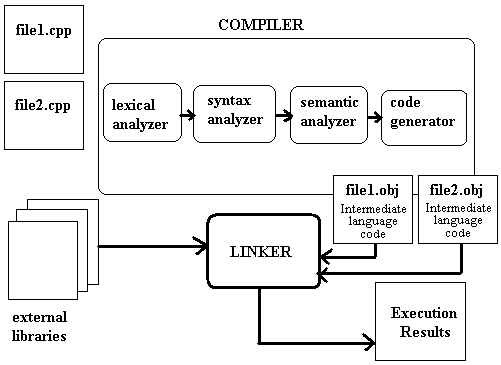
\includegraphics[scale=0.5]{compile.png}
\end{frame}
%--------------------------------------------------------------------------
\subsection{Java Process}
\begin{frame}
\frametitle{Java Process}
\begin{itemize}
\item Uses a {\color{red} Hybrid compiler-interpreter} method.
\item Compiles source nto {\color{green} byte code}.
\item {\color{green} Byte code} is portable.
\item When a class ({\color{green} byte code} file) is executed, the JVM {\color{orange} compiles} and {\color{purple} executes} it.
\item Known as {\color{magenta} Just In Time} compilation.
\item Main method can change without recompiling the bytecode, since everything is compiled on the fly.
\end{itemize}
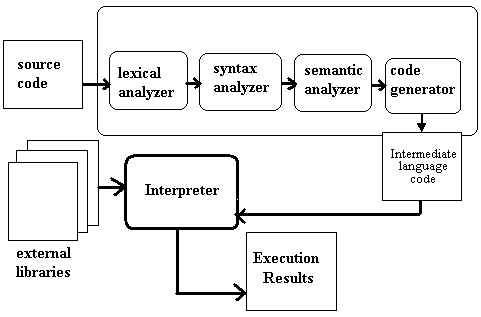
\includegraphics[scale=0.3]{inter.png}
\end{frame}
%--------------------------------------------------------------------------
\subsection{C\# Process}
\begin{frame}
\frametitle{C\# Process}
\begin{itemize}
\item C\# is compiled into {\color{red} IL} equivalent to bytecode, but unit of compilation is in {\color{green} assembly (DLL file)}.
\item This means if the main method changes then the whole project has to be recompiled.
\item {\color{purple} .NET} then converts the assembly code into executables.
\item The {\color{orange} CLR} is an environment in which the {\color{purple} .NET} applications that have been compiled to {\color{red} IL} can be run. 
\item Does not interpret. It forms an {\color{magenta}executable}.
\end{itemize}
\end{frame}
%-----------------------------------------------------------------------------
\defverbatim[colored]\inher{
\begin{lstlisting}[style = customc, basicstyle=\scriptsize]
class Class1 {}
interface IMyInterface{}
class Class 2: Class1, IMyInterface {} 
\end{lstlisting}
}
\section{Engineering Concepts}
\subsection{Inheritance}
\begin{frame}
\frametitle{Inheritance}
\inher
\begin{itemize}
\item Uses c++ style to signify inheritance using a \texttt{:}.
\item It is not obvious which class is inherited and which are implemented interfaces. 
\item By convention interfaces being with an I.
\item Only {\color{green} single inheritance} is allowed.
\item All objects inherit from base class {\color{red} object}.
\item The operator \texttt{is} is the equivalent to \texttt{instanceof} in java.
\item Made unextendable with the keyword \texttt{sealed}.
\end{itemize}
\end{frame}
%--------------------------------------------------------------
\defverbatim[colored]\over{
\begin{lstlisting}[style = customc, basicstyle=\tiny]
public class Mammal { 
 virtual public void move(){// Overridden or shadowed
  Console.WriteLine("Move like a mammal in C#");}
 virtual public void jump(){ // Overridden or shadowed
  Console.WriteLine("Jump like an mammal in C#");  }
 public void dance(){ // Shadowed only
  Console.WriteLine("dance like a mammalin C#"); }
}
--------------------------------------------------------
public class Dog : Mammal{
  override public void move(){ // Overrides method
     Console.WriteLine("Move like a dog in C#");}
   public void jump(){ // Shadows - Static type decides on method called
     Console.WriteLine("Jump like a dog in C#");}
   public void dance(){ // Shadows - Static type decides on method called
     Console.WriteLine("Dance like a dog in C#");}
}
\end{lstlisting}
}
\subsubsection{Method overriding}
\begin{frame}
\frametitle{Method Overriding}
\begin{itemize}
\item By default, methods cannot be overridden, they must be declared as \texttt{\color{red} virtual}.
\item Methods can be {\color{green}shadowed} (Method called the same name, but not {\color{orange} overridden}, static type determines method called).
\item {\color{red}Virtual} methods can be {\color{orange}overridden} or {\color{green} shadowed}.
\item To {\color{orange} override} then the keyword \texttt{override} must be used, otherwise it is {\color{green} shadowed}.
\end{itemize}
\over
\end{frame}
%--------------------------------------------------------------------------------
\defverbatim[colored]\ex{
\begin{lstlisting}[style = customc, basicstyle=\tiny]
 class Cat : Mammal
    {
        override public void jump(){
            Console.WriteLine("Jump like a Cat");}
	  public void move(){
            Console.WriteLine("Move like a Cat");} }
----------------------------------------------------------
 static void Main(string[] args)
 {
    Dog rover= new Dog();
    Cat mog = new Cat();
    Mammal mammal= new Mammal();
    Mammal myPet = rover; // Static - Mammal, Dynamic - Dog
    
    mammal.move();
	rover.move();
	mog.move();
	myPet.move();
	myPet=mog;
	myPet.move();
--------------------------------------------------------
// Output:
// Move like an animal
// Move like a dog
// Move like a cat

// Type of My Pet = Dog
// Move like a dog

// Type of My Pet = Cat
// Move like a Mammal
}
\end{lstlisting}
}
\begin{frame}
\frametitle{Method Overriding - Cont}
\ex
\end{frame}
%---------------------------------------------------------------------------------
\subsubsection{Summary}
\begin{frame}
\frametitle{Summary}
\begin{itemize}
\item Interfaces and Abstract methods are the same as in Java.
\item Don't shadow methods, bad form.
\item In Java/C\# all objects inherit from a common base class (\texttt{Object/object}), in C++, they don't.
\item {\color{green} C++ allows multiple inheritance} {\color{red} Java/C\# Do not}.
\item By default, methods in C++ and C\# cannot be overridden. Must be explicitly declared as \texttt{virtual}. Java can always be overridden unless stated as \texttt{final}.
\item C++ and C\# allow method shadowing... for some reason... who knows why?
\end{itemize}
\end{frame}
%-----------------------------------------------------------------------------------
\defverbatim[colored,width = .5\textwidth]\sto{
\begin{lstlisting}[style = customc, basicstyle=\tiny]
struct point {
	byte x;
	byte y;
}
\end{lstlisting}
}

\defverbatim[colored,width = .5\textwidth]\clas{
\begin{lstlisting}[style = customc, basicstyle=\tiny]
class point2 {
	byte x;
	byte y;
}
\end{lstlisting}
}
\defverbatim[colored]\after{
\begin{lstlisting}[style = customc, basicstyle=\tiny]
Point[] myPoints = new Point[1000000];// 2 Million bytes allocated on stack
Point2[] mP2 = new Point2[1000000]; // 1 Million bytes allocated on stack the 2 million on Heap
\end{lstlisting}
}
\subsection{Design Components}
\subsubsection{Structs}
\begin{frame}
\frametitle{Structs}
\begin{itemize}
\item C\# allows C like \texttt{struct}s.
\item These are {\color{green} value} types and not {\color{red} reference} types like classes are.
\item The name of the struct variable is directly associated with the data and allocated on the {\color{red} stack} rather than the heap.
\item No inheritance.
\item Useful for large, structured {\color{purple} immutable} data.
\item Main benefit is that they do not need a reference to point to them and the memory is allocated at compile time which can be more efficient.
\end{itemize}
\begin{columns}[t]
\column{.5\textwidth}
\sto
\column{.5\textwidth}
\clas
\end{columns}
\after
\end{frame}
%-----------------------------------------------------------------------------
\subsubsection{Unsafe C\#}
\begin{frame}
\frametitle{Unsafe C\#}
\begin{itemize}
\item C\# hides most of its memory management like Java.
\item Possible to do C like {\color{red}pointer manipulation} in C\# if you are in an \texttt{unsafe} block or method.
\item Must be compiled with the unsafe flag set.
\item Bypasses all memory checking and management done by the CLR.
\item Can have \texttt{unsafe struct}s too.
\item Again, bad form, stick to C.
\end{itemize}
\end{frame}
%----------------------------------------------------------------------------------
\subsubsection{Memory Management}
\begin{frame}
\frametitle{Memory Management}
\begin{itemize}
\item Constructors are the same as in Java.
\item Can also have destructors in C\#. Same syntax as C++.
\item Semantics are like Java finalizers, but more useful.
\end{itemize}
\end{frame}
%----------------------------------------------------------------------------
\defverbatim[colored]\generics{
\begin{lstlisting}[style = customc, basicstyle=\tiny]
public struct Point<T> {
 public T x;
 public T y;
 public Point(T a, T b){
  x = a;
  y = b;
 }
}
-------------------------------------------
using System.Collections.Generic.List;
static void genericTest(){

 List<string> myList = List<string>();
 List<Point<int>> points=new List<Point<int>>();
 myList.Add("Up the Arsenal");
 points.Add(new Point<int>(1, 2));
}
\end{lstlisting}
}
\subsubsection{Generics/Templates}
\begin{frame}
\frametitle{Generics/Templates}
\begin{itemize}
\item C++ uses {\color{green} Code specialization}
\item Java uses {\color{red} Type erasure}
\item C\# performs {\color{green} code specialization} for primitives (at second compilation phase).
\item C\# performs {\color{red} Type erasure} for reference types.
\item Syntactically, the same as Java, however you can have primitives and hence struct generics.
\end{itemize}
\generics
\end{frame}
%--------------------------------------------------------------------------------
\subsubsection{Nested classes/Enums}
\begin{frame}
\frametitle{Nested Classes/Enums}
\begin{itemize}
\item Nested classes:
\begin{itemize}
\item C\# has the equivalent to Java static nested classes.
\item No equivalent for local inner classes, anonymous classes or inner classes.
\end{itemize}
\item Enums:
\begin{itemize}
\item C\# enums are simply masked integers like in C/C++.
\end{itemize}
\end{itemize}
\end{frame}
%--------------------------------------------------------------------------------
\defverbatim[colored]\iter{
\begin{lstlisting}[style = customc, basicstyle=\tiny]
IEnumerator<string> iterator = myList.GetEnumerator();
while (iterator.Current != null) // Gets current element
{
	Console.WriteLine(iterator.Current);
	iterator.MoveNext(); // Moves to next element
}
\end{lstlisting}
}
\subsection{Collections}
\begin{frame}
\frametitle{Collections}
\scriptsize
\begin{itemize}
\item \texttt{System.Collections} or \texttt{System.Collections.Generic}
\item Lists:
\begin{itemize}
\scriptsize
\item \texttt{ArrayList}
\item \texttt{LinkedList}
\item \texttt{SortedList}
\item \texttt{BitList}
\item \texttt{Stack and Queue}
\end{itemize}
\item Set:
\begin{itemize}
\scriptsize
\item \texttt{HashSet}
\item \texttt{SortedSet}
\end{itemize}
\item Maps:
\begin{itemize}
\scriptsize
\item \texttt{Dictionary Classes}
\item \texttt{HashTable}
\item \textbf{No \texttt{TreeMap}}
\end{itemize}
\item Iterating:
\begin{itemize}
\scriptsize
\item Any class that implements the \texttt{IEnumerable} interface can be using in a \texttt{foreach} context.
\iter
\end{itemize}
\end{itemize}
\end{frame}
%---------------------------------------------------------------------------------
\subsubsection{Sorting}
\begin{frame}
\frametitle{Sorting}
\begin{itemize}
\item \texttt{Collections} has a default sort, to use it on a class, the class must implement \texttt{IComparable}.
\item Java uses {\color{red} Functors} to sort by another method than the default, C\# uses {\color{green} Delegates}.
\item {\color{green} Delegates} are a form of method pointer and hence can be used instead of {\color{red} Functors}.
\end{itemize}
\end{frame}
%----------------------------------------------------------------------------
\defverbatim[colored]\delo{
\begin{lstlisting}[style = customc, basicstyle=\tiny]
public delegate int CompareStudent(Student s);
public delegate int StaticCompare (Student a, Student b);
\end{lstlisting}
}
\defverbatim[colored]\delt{
\begin{lstlisting}[style = customc, basicstyle=\tiny]
public int compNos(Student s)
{
  if (nos > s.nos)   
    return 1;
  if (nos < s.nos)  
    return -1;
  return 0;
}
-----------------------------------------
public int compName(Student s)
{
  return name.CompareTo(s.name);
}
\end{lstlisting}
}

\defverbatim[colored]\delth{
\begin{lstlisting}[style = customc, basicstyle=\tiny]
// Declare two delegate references
Student.CompareStudent objectMethodPointer;
Student.StaticCompareStudent staticMethodPointer;

// Assign methods to them
objectMethodPointer = bob.CompNos;
staticMethodPointer =Student.CompNos;

// Call methods via delegate
int x = objectMethodPointer.Invoke(alice);
int y = staticMethodPointer.Invoke(bob, alice);

objectMethodPointer = alice.CompName;
staticMethodPointer = Student.CompName;
x = objectMethodPointer.Invoke(bob);
y = staticMethodPointer.Invoke(bob, alice);
\end{lstlisting}
}
\defverbatim[colored]\exam{
\begin{lstlisting}[style = customc, basicstyle=\tiny]
myClass.findBest(
new Student.StaticCompareStudent(Student.CompNos)
);
\end{lstlisting}
}
\subsubsection{Delegates}
\begin{frame}[allowframebreaks]
\frametitle{Delegates}
\begin{enumerate}
\item Declare \texttt{delegate} with a specific signature:
\delo
\item Write methods that could be stores in a delegate:
\delt
\item Now possible to declare a \texttt{delegate} and store a pointer to different functions:
\delth
\end{enumerate}
\begin{itemize}
\item Often passed to methods to act as a form of selection.
\item Often created at the method call in a similar way to anonymous inner classes:	
\exam
\end{itemize}
\end{frame}
%-------------------------------------------------------------------------
\defverbatim[colored]\lam{
\begin{lstlisting}[style = customc, basicstyle=\tiny]
int square(int x) {return x*x;}
// Is the same as:
x=>x*x; // Lambda form
);
\end{lstlisting}
}
\defverbatim[colored]\lamt{
\begin{lstlisting}[style = customc, basicstyle=\tiny]
delegate int del(int i); 
static void Main(string[] args) { 
     del myDelegate = x => x * x; 
     int j = myDelegate(5); //j = 25 
}
\end{lstlisting}
}
\subsubsection{Lambdas}
\begin{frame}
\begin{itemize}
\item They are a form of anonymous function.
\lam
\item Lambdas can be stored as \texttt{delegates}:
\lamt
\end{itemize}
\end{frame}
%-------------------------------------------------------------
\section{Differences Between Languages}
\begin{frame}
\frametitle{Differences Between Languages}
\scriptsize
\begin{itemize}
\item \textbf{Inheritance:} In Java/C\# all objects inherit from a common base class (\texttt{Object/object}).
\item \textbf{Inheritance:} C++ allows {\color{red} Multiple inheritance}, Java and C\# do not,
\item \textbf{Inheritance:} By default, methods in C++ and C\# cannot be overridden, they must be explicitly declared as \texttt{\color{green}virtual}. In Java they can always be overridden unless \texttt{final}.
\item \textbf{Nested Classes:} Java has four types, C\#/C++ only has static nested classes.
\item \textbf{Enum:} Java enums are instances of anonymous inner classes, C++/C\# are wrappers for integers.
\item \textbf{Structs:} C++/C\# allow structs (User defined primitives).
\item \textbf{Generics/Templates:} Java uses {\color{orange} Type erasure}, C++ uses {\color{magenta} Code specialization}, C\# uses {\color{orange} Type erasure} for objects and {\color{magenta} Code specialization} for primitives.
\item \textbf{Threads:} Java/C\# have built in threads, C++ does not.
\item \textbf{Passing methods:} Java uses functors, C++ uses function pointers and C\# uses Delegates
\item \textbf{Operator overloading:} Allowed in C\#/C++, not allowed in Java.
\end{itemize}
\end{frame}
%----------------------------------------------------------------------------------
\begin{frame}
\Huge{\centerline{The End}}
\end{frame}

%----------------------------------------------------------------------------------------

\end{document}